\documentclass[conference]{IEEEtran}
\IEEEoverridecommandlockouts

\usepackage{cite}
\usepackage{amsmath,amssymb,amsfonts,amsthm}
\usepackage{graphicx}
\usepackage{booktabs}
\usepackage{textcomp}
\usepackage{xcolor}
\usepackage{url}
\usepackage[hidelinks]{hyperref}
\usepackage{orcidlink}

\newtheorem{proposition}{Proposition}
\newcommand{\ket}[1]{\left|#1\right\rangle}
\newcommand{\bra}[1]{\left\langle#1\right|}
\newcommand{\cpla}{CPLA}

\begin{document}

\title{From Quantum Fidelity to Linear-Time Attention:\\
An Exact Classical Reduction of Quantum Self-Attention}

\author{\IEEEauthorblockN{Chandra Sekhar Singuru\,\orcidlink{0009-0004-0219-1960}}
\IEEEauthorblockA{\textit{Independent Researcher}\\
Long Beach, CA, USA\\
sekharc669@gmail.com\\
ORCID: 0009-0004-0219-1960}
}

\maketitle

\begin{abstract}
Quantum self-attention models replace the Transformer's dot-product score with the fidelity between quantum states that encode two tokens. We ask where the accuracy gains reported for such models come from, and whether they require a quantum computer. We show analytically that, for angle-encoded states, the fidelity score equals a classical cosine-product (CP) kernel, and that any fidelity-based attention admits an explicit feature map of dimension $4^n$ for $n$ qubits. The second result yields cosine-product linear attention (\cpla), a classical layer whose cost grows linearly with sequence length. We compare nine attention variants, including a quantum layer implemented with the Qiskit Estimator and trained with exact parameter-shift gradients, on three token-matching tasks over five seeds and on the SST-2 sentiment benchmark. The quantum layer beats dot-product attention by 0.13 to 0.31 accuracy on matching tasks, but the classical CP kernel matches it within seed variance, and \cpla{} matches or exceeds it on two of three tasks while running about 22$\times$ faster than softmax attention at 4{,}096 tokens. Widening the dot-product baseline or using standard linear attention does not close the gap. On SST-2, by contrast, dot-product attention is best and all cosine-product layers, quantum or classical, trail it by 1.2 to 2.4 points, showing that the kernel suits matching-type structure rather than graded similarity. We further find that gradient variance of the quantum layer decays roughly exponentially with qubit count, and that accuracy degrades under simulated shot noise. The useful contribution of quantum self-attention, in this regime, is a kernel that classical Transformers can adopt directly.
\end{abstract}

\begin{IEEEkeywords}
attention mechanism, Transformers, linear attention, kernel methods, quantum machine learning, quantum kernels, parameterized quantum circuits, barren plateaus
\end{IEEEkeywords}

% ===========================================================================
\section{Introduction}
% ===========================================================================

Attention lets each token in a Transformer weigh every other token, and its standard score is a scaled dot product of learned query and key projections~\cite{vaswani2017attention}. Viewed as a kernel smoother~\cite{tsai2019dissection}, attention is defined by its similarity function, and changing that function has driven much of the work on efficient Transformers~\cite{katharopoulos2020linear,choromanski2021performer,qin2022cosformer}.

Quantum machine learning offers a new family of similarity functions. Encoding two inputs as quantum states and measuring their overlap gives a quantum kernel~\cite{havlicek2019supervised,schuld2019feature}. Several recent models use such overlaps as attention scores~\cite{li2024qsann,zhao2024qksan,chen2024qmsan}, and a recent survey reports preliminary advantages on small tasks~\cite{zhang2025survey}. Two questions are rarely tested directly. First, does the reported gain come from quantum effects or from the shape of the kernel? Second, does fidelity attention have to cost one circuit per token pair?

We answer both, analytically and empirically. Our contributions are:
\begin{enumerate}
  \item \textbf{An exact classical reduction.} For angle-encoded states the fidelity score is a cosine-product (CP) kernel (Proposition~\ref{prop:cp}). More generally, any fidelity attention is an inner product of explicit $4^n$-dimensional features (Proposition~\ref{prop:lin}).
  \item \textbf{A linear-time attention layer.} Proposition~\ref{prop:lin} yields cosine-product linear attention (\cpla), whose cost grows linearly in sequence length $N$.
  \item \textbf{A controlled comparison.} We evaluate nine attention variants, from a quantum layer with exact parameter-shift gradients to wide dot-product and standard linear attention, on three token-matching tasks and on SST-2~\cite{socher2013sst}.
  \item \textbf{Scaling limits of the quantum layer.} We measure gradient variance versus qubit count, accuracy versus register size, and robustness to shot noise.
\end{enumerate}

The results are consistent across all four. The quantum layer's advantage over dot-product attention on matching tasks is real, but it is fully reproduced by the classical CP kernel, and \cpla{} delivers it in linear time. On natural-language sentiment classification, dot-product attention remains best, which delimits where the kernel helps.

% ===========================================================================
\section{Related Work}
% ===========================================================================

\subsection{Kernel Views and Efficient Attention}
Tsai \emph{et al.}~\cite{tsai2019dissection} cast attention as a kernel smoother, separating the choice of similarity function from the rest of the layer. Linear attention~\cite{katharopoulos2020linear} replaces the softmax with a positive feature map $\phi$, so that $\sum_j \phi(q_i)^\top\phi(k_j)v_j$ can be computed in time linear in $N$. Performers~\cite{choromanski2021performer} approximate the softmax kernel with random features, and cosFormer~\cite{qin2022cosformer} keeps attention linear while modulating scores with a cosine function of token distance, which sharpens the attention distribution. \cpla{} belongs to this family, with an exact rather than approximate feature map derived from a quantum circuit.

\subsection{Quantum Self-Attention}
QSANN~\cite{li2024qsann} measures one Pauli-$Z$ expectation per query and key and scores them with a Gaussian of their difference. QKSAN~\cite{zhao2024qksan} computes attention from quantum kernel overlaps, and QMSAN~\cite{chen2024qmsan} uses swap tests between mixed-state queries and keys, with similarity $\operatorname{tr}(\rho\sigma)$. Quantum vision Transformers~\cite{cherrat2024qvt} use matrix-loading circuits and orthogonal layers, and Quixer~\cite{khatri2024quixer} builds token superpositions with linear combinations of unitaries. SASQuaTCh~\cite{evans2025sasquatch} realizes attention as a trainable kernel applied in the quantum Fourier domain. Tomal \emph{et al.}~\cite{tomal2025qiattn} score tokens with dot products of measured quantum features plus an interference term, and compare against standard dot-product attention but not against a classical kernel of the same form. Pecilli and Rosati~\cite{pecilli2026overlap} drop the softmax and obtain gate complexity linear in sequence length for an overlap-based quantum attention. The survey of Zhang \emph{et al.}~\cite{zhang2025survey} observes that pairwise quantum attention keeps the quadratic dependence on the number of tokens. Our analysis applies to the overlap-based models: both the pure-state fidelity and $\operatorname{tr}(\rho\sigma)$ satisfy Proposition~\ref{prop:lin}.

\subsection{Quantum Kernels and Classical Simulability}
Fidelity kernels were introduced as quantum-enhanced feature spaces~\cite{havlicek2019supervised,schuld2019feature}. Circuits that encode data through Pauli rotations compute trigonometric polynomials whose frequencies are fixed by the encoding~\cite{schuld2021encoding}, which allows classical surrogate models to stand in for them in many cases~\cite{schreiber2023surrogates}. Shin \emph{et al.}~\cite{shin2023dequantizing} relate variational quantum models to matrix product states and derive efficient classical kernels from quantum ones. Our reduction is in the same spirit but specific to attention: it gives the exact closed form of the score and turns it into a linear-time layer. Systematic benchmarks have found no consistent advantage of quantum models over classical baselines~\cite{bowles2024benchmarking}. On the trainability side, random circuits suffer barren plateaus~\cite{mcclean2018barren}, global cost functions suffer them even at shallow depth~\cite{cerezo2021cost}, quantum kernel values can concentrate exponentially~\cite{thanasilp2024concentration}, and provable absence of barren plateaus often coincides with classical simulability~\cite{cerezo2025simulability}. Our results instantiate these concerns concretely for attention.

% ===========================================================================
\section{Fidelity Attention and Its Classical Reduction}
% ===========================================================================

\subsection{Quantum Fidelity Attention}
Each token embedding $x\in\mathbb{R}^d$ is mapped to $n$ angles $\phi(x)=\pi\tanh(Ax)$ with a learned $A\in\mathbb{R}^{n\times d}$, and encoded by $R_Y$ rotations:
\begin{equation}
S(\phi)\ket{0}^{\otimes n} = \bigotimes_{k=1}^{n}\left(\cos\tfrac{\phi_k}{2}\ket{0} + \sin\tfrac{\phi_k}{2}\ket{1}\right).
\label{eq:encode}
\end{equation}
Separate hardware-efficient ansatzes $W_Q(\theta_Q)$ and $W_K(\theta_K)$, each with $L$ layers of $R_Y$ rotations and a CNOT ring, form the query and key states $\ket{\psi_Q(x)}=W_Q S(\phi(x))\ket{0}$ and $\ket{\psi_K(x)}=W_K S(\phi(x))\ket{0}$. The score is their fidelity, estimated with the compute--uncompute circuit of Fig.~\ref{fig:circuit}:
\begin{equation}
s_{ij} = \left|\langle\psi_K(x_j)|\psi_Q(x_i)\rangle\right|^2 = \bra{0}U_{ij}^\dagger P_0 U_{ij}\ket{0},
\end{equation}
where $U_{ij}=S(\phi_j)^\dagger W_K^\dagger W_Q S(\phi_i)$ and $P_0=\ket{0}\!\bra{0}^{\otimes n}$. We evaluate $P_0$ as a sum of $2^n$ Pauli-$Z$ strings with the Qiskit Estimator V2 primitive~\cite{qiskit2024}. Attention weights are $a_{ij}=\operatorname{softmax}_j(\beta s_{ij})$ with learned $\beta$, and the output is $y_i=W_O\sum_j a_{ij}W_V x_j$.

Every parameter enters through one $R_Y$ gate, so gradients follow the exact parameter-shift rule $\partial s/\partial a=\frac12[s(a+\frac{\pi}{2})-s(a-\frac{\pi}{2})]$~\cite{schuld2019gradients}. We implement this as a PyTorch~\cite{paszke2019pytorch} autograd function that batches all shifted circuits into one Estimator call.

\begin{figure}[t]
\centering
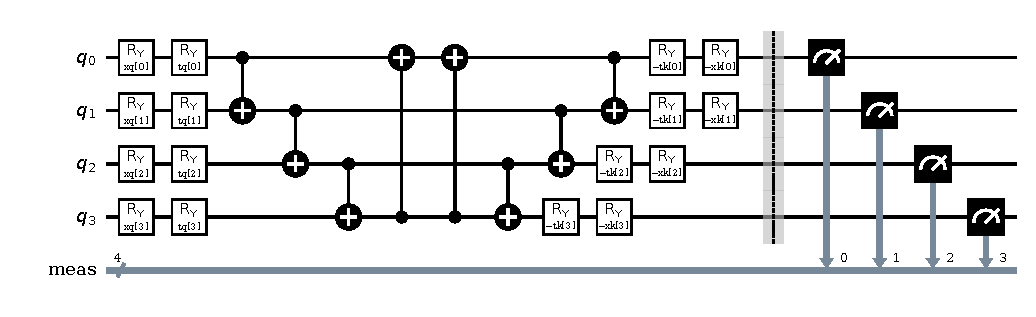
\includegraphics[width=\columnwidth]{figures/circuit.pdf}
\caption{Compute--uncompute circuit for one score $s_{ij}$ ($n=4$, $L=1$): encoding of token $i$ ($x_q$), query ansatz $W_Q$ ($t_q$), inverse key ansatz ($-t_k$), inverse encoding of token $j$ ($-x_k$). The probability of $\ket{0000}$ equals the fidelity.}
\label{fig:circuit}
\end{figure}

\subsection{Exact Classical Reduction}

\begin{proposition}[Cosine-product kernel]\label{prop:cp}
Without an ansatz ($W_Q=W_K=I$), the fidelity of the states in \eqref{eq:encode} is
\begin{equation}
s_{ij} = \prod_{k=1}^{n}\cos^2\!\left(\frac{\phi_{ik}-\phi_{jk}}{2}\right).
\label{eq:cp}
\end{equation}
\end{proposition}
\begin{proof}
The states are real tensor products, so the overlap factorizes: $\prod_k\left(\cos\frac{\phi_{ik}}{2}\cos\frac{\phi_{jk}}{2}+\sin\frac{\phi_{ik}}{2}\sin\frac{\phi_{jk}}{2}\right)=\prod_k\cos\frac{\phi_{ik}-\phi_{jk}}{2}$. Squaring gives \eqref{eq:cp}.
\end{proof}

The trained model is close to this kernel in practice. With small initial angles, $W_K^\dagger W_Q = I + O(\theta)$ because the CNOT layers of the two ansatzes cancel, so at initialization the quantum layer computes \eqref{eq:cp} up to a small perturbation.

\begin{proposition}[Exact linearization]\label{prop:lin}
For any $n$-qubit states $\ket{\psi_Q(x)}$, $\ket{\psi_K(x)}$, let $\Phi_Q(x)=\operatorname{vec}(\ket{\psi_Q}\!\bra{\psi_Q})$ and likewise $\Phi_K$. Then $s_{ij}=\langle\Phi_Q(x_i),\Phi_K(x_j)\rangle$, an inner product in $\mathbb{C}^{4^n}$ that is real and non-negative. Consequently, normalized fidelity attention
\begin{equation}
y_i=\frac{\sum_j s_{ij}\,v_j}{\sum_j s_{ij}}=\frac{\Phi_Q(x_i)^{\!\top}\big(\sum_j \Phi_K(x_j)v_j^\top\big)}{\Phi_Q(x_i)^{\!\top}\sum_j \Phi_K(x_j)}
\label{eq:linear}
\end{equation}
can be computed in $O(N\,4^n d)$ time and $O(4^n d)$ memory, given the states.
\end{proposition}
\begin{proof}
$|\langle a|b\rangle|^2=\langle a|b\rangle\langle b|a\rangle=\operatorname{tr}(\ket{a}\!\bra{a}\,\ket{b}\!\bra{b})$, which is the Hilbert--Schmidt inner product of two Hermitian matrices. Reassociating the sums in \eqref{eq:linear} gives the stated cost~\cite{katharopoulos2020linear}.
\end{proof}

For real states, as produced by $R_Y$ and CNOT gates, $\Phi(x)=\psi(x)\otimes\psi(x)$. The same argument covers mixed-state similarity $\operatorname{tr}(\rho\sigma)$~\cite{chen2024qmsan}. Proposition~\ref{prop:lin} has a notable consequence: on quantum hardware, fidelity attention needs one overlap circuit per token pair, $N^2$ in total, whereas a classical simulation of the same layer needs only $N$ state preparations. For small $n$, simulating the quantum model is asymptotically cheaper in $N$ than running it.

\subsection{Cosine-Product Linear Attention}
Combining both propositions gives \cpla. With $\psi(x)=\bigotimes_k[\cos\frac{\phi_k(x)}{2},\sin\frac{\phi_k(x)}{2}]\in\mathbb{R}^{2^n}$ and $\Phi(x)=\psi(x)\otimes\psi(x)\in\mathbb{R}^{4^n}$, \cpla{} evaluates \eqref{eq:linear} with $\Phi_Q=\Phi_K=\Phi$. It computes the CP kernel exactly, needs no quantum hardware, and has $nd+n$ score parameters. Unlike softmax attention it has no temperature; the sharpness of the kernel is controlled by the learned encoding scale.

\textit{Remark.} For real $\psi$ the vector $\psi\otimes\psi$ is redundant: its entries for each qubit pair are symmetric, so the CP kernel needs fewer than $4^n$ features. Writing $\cos^2\frac{a-b}{2}=\frac12(1+\cos a\cos b+\sin a\sin b)$ shows that the per-qubit map $\frac{1}{\sqrt2}[1,\cos\phi_k,\sin\phi_k]$ already reproduces \eqref{eq:cp} exactly, giving $3^n$ features. A companion paper~\cite{singuru2026cost} develops this reduction and uses it to bound the training cost of quantum attention; here we keep the general $4^n$ map of Proposition~\ref{prop:lin}, which also covers trained ansatz states.

Table~\ref{tab:cost} summarizes the costs. For a fixed small $n$, \cpla{} is linear in $N$; its constant $4^n$ ($3^n$ with the remark above) limits it to registers of roughly 4 to 6 qubits, which is the regime where the quantum layer also trains best (Section~\ref{sec:trainability}).

\begin{table}[t]
\caption{Cost per Sequence of Length $N$ (Embedding Width $d$)}
\label{tab:cost}
\centering
\setlength{\tabcolsep}{3pt}
\begin{tabular}{@{}lll@{}}
\toprule
Attention layer & Time & Notes \\
\midrule
Softmax dot product & $O(N^2 d)$ & exact \\
Quantum fidelity (QPU) & $N^2$ circuits & $O(1/\varepsilon^2)$ shots each \\
Quantum fidelity (simulated) & $O(N 2^n nL + N^2 2^n)$ & pairwise softmax \\
CP kernel, softmax & $O(N^2 2^n)$ & exact, classical \\
\cpla{} (ours) & $O(N 4^n d)$ & exact, classical \\
Linear attn., elu+1~\cite{katharopoulos2020linear} & $O(N d_k d)$ & exact \\
\bottomrule
\end{tabular}
\end{table}

% ===========================================================================
\section{Experimental Setup}
% ===========================================================================

\subsection{Tasks}
\textit{Token matching.} Three synthetic tasks require comparing tokens with one another (Table~\ref{tab:tasks}). Sequences are drawn from a vocabulary of 12 random 16-dimensional embeddings with Gaussian noise ($\sigma=0.1$) added to every token. For each seed we draw a vocabulary and then 512 balanced training and 512 held-out test sequences from it.

\textit{Sentiment.} SST-2~\cite{socher2013sst} has 6{,}920 training, 872 development and 1{,}821 test sentences. We lowercase, keep words seen at least twice in training (7{,}206 tokens including padding and unknown), and truncate to 48 tokens.

\begin{table}[t]
\caption{Token-Matching Tasks}
\label{tab:tasks}
\centering
\setlength{\tabcolsep}{3pt}
\begin{tabular}{@{}lcl@{}}
\toprule
Task & $N$ & Positive label when \\
\midrule
repeat & 6 & any token occurs twice \\
match-first & 6 & token 0 recurs; negatives hold a decoy repeat \\
two-pairs & 8 & two tokens each occur twice; negatives have one \\
\bottomrule
\end{tabular}
\end{table}

\subsection{Model and Attention Variants}
Every model adds a learned positional embedding, applies one residual attention layer and layer normalization, max-pools over tokens and classifies with a two-layer MLP. Only the attention layer changes. We compare: the quantum fidelity layer ($n=4$, $L=2$); the same with frozen $\theta$; the CP kernel with softmax; \cpla; an RBF kernel $\exp(-\|q_i-k_j\|^2)$; dot-product attention with $d_k=4$ and $d_k=16$; linear attention with elu$+1$ features~\cite{katharopoulos2020linear} ($d_k=16$); and no attention. All kernel-based layers compress to 4 features, matching the qubit count; the $d_k=16$ variants give the dot-product and linear baselines four times more query/key capacity. Attention-layer parameter counts on the synthetic tasks ($d=16$) are 629, 613, 613, 612, 681, 680, 1{,}088, 1{,}088 and 0, of which 544 are the shared value and output projections.

\subsection{Training and Simulation}
On synthetic tasks we train with Adam (learning rate $10^{-2}$, batch 32) for 60 epochs, over five seeds. On SST-2 we use $d=64$, dropout 0.3 on embeddings, Adam (learning rate $10^{-3}$, weight decay $10^{-5}$, batch 64) for 10 epochs, five seeds, and report test accuracy at the epoch with the best development accuracy.

Experiments use an exact PyTorch statevector simulation of the circuit. All gates are real, so states are real vectors and automatic differentiation gives exact gradients. The simulator matches the Qiskit Estimator and parameter-shift implementation to within $10^{-15}$ in scores and gradients for $(n,L)\in\{(2,1),(2,2),(3,2),(4,2),(6,3)\}$, and the \cpla{} feature map reproduces \eqref{eq:cp} to within $10^{-15}$.

\subsection{Shot-Noise Model}
A score is a probability $p$ estimated from shots with standard error at most $1/(2\sqrt{\text{shots}})$. We add Gaussian noise with standard deviation $\varepsilon\in\{0,0.01,0.03,0.1,0.3\}$ to every score during training and testing, clipped to $[0,1]$, covering roughly 2{,}500 down to 3 shots per score. Gradients pass through the clean score.

% ===========================================================================
\section{Results}
\label{sec:results}
% ===========================================================================

\subsection{Token Matching}

\begin{figure*}[t]
\centering
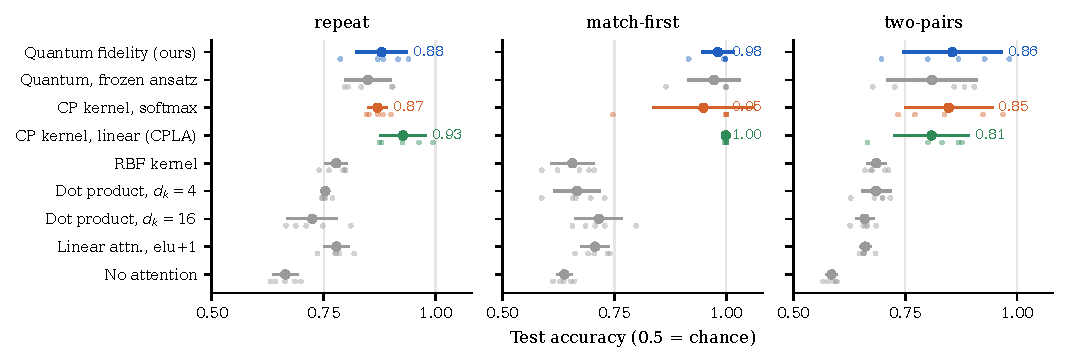
\includegraphics[width=\textwidth]{figures/accuracy.pdf}
\caption{Held-out accuracy on three token-matching tasks: mean $\pm$ one standard deviation over five seeds (large markers) and individual seeds (small markers). The classical CP kernel (orange) and its linear-time form \cpla{} (green) match the quantum layer (blue); wider dot-product and standard linear attention do not.}
\label{fig:accuracy}
\end{figure*}

\begin{table}[t]
\caption{Token-Matching Test Accuracy (Mean $\pm$ Std., 5 Seeds)}
\label{tab:accuracy}
\centering
\setlength{\tabcolsep}{2.5pt}
\begin{tabular}{@{}lccc@{}}
\toprule
Attention layer & repeat & match-first & two-pairs \\
\midrule
Quantum fidelity       & .879$\pm$.058 & .981$\pm$.036 & \textbf{.855}$\pm$.111 \\
Quantum, frozen        & .848$\pm$.052 & .972$\pm$.060 & .810$\pm$.101 \\
CP kernel, softmax     & .870$\pm$.022 & .949$\pm$.113 & .847$\pm$.099 \\
\cpla{} (linear)       & \textbf{.927}$\pm$.052 & \textbf{.999}$\pm$.002 & .809$\pm$.086 \\
RBF kernel             & .778$\pm$.026 & .656$\pm$.049 & .686$\pm$.022 \\
Dot product, $d_k{=}4$ & .754$\pm$.009 & .667$\pm$.053 & .685$\pm$.034 \\
Dot product, $d_k{=}16$& .725$\pm$.057 & .715$\pm$.054 & .659$\pm$.021 \\
Linear, elu$+1$        & .779$\pm$.029 & .707$\pm$.032 & .661$\pm$.013 \\
No attention           & .664$\pm$.029 & .638$\pm$.019 & .586$\pm$.013 \\
\bottomrule
\end{tabular}
\end{table}

Fig.~\ref{fig:accuracy} and Table~\ref{tab:accuracy} give the main comparison. The quantum layer beats dot-product attention ($d_k=4$) by 0.13, 0.31 and 0.17 on repeat, match-first and two-pairs (mean paired difference per seed). Quadrupling the dot-product width does not help: against $d_k=16$ the gaps are 0.16, 0.27 and 0.20. Standard linear attention performs like the dot product.

The gain is not quantum in origin. Against the classical CP kernel, the paired differences are 0.01, 0.03 and 0.01, each smaller than its standard deviation across seeds (0.07, 0.13 and 0.14). Freezing the ansatz costs 0.01 to 0.05, within seed variance, as Proposition~\ref{prop:cp} and the near-identity initialization predict. \cpla{} reaches 0.93 and 0.999 on repeat and match-first, above the quantum layer, and 0.81 on two-pairs, below it by 0.05 but within one standard deviation. An RBF kernel, also bounded and maximal at identical inputs, does not reproduce the gain, which points to the periodic, per-feature product form of \eqref{eq:cp}.

\subsection{Natural-Language Sentiment}

\begin{table}[t]
\caption{SST-2 Accuracy (Mean $\pm$ Std., 5 Seeds; Test at Best Dev Epoch)}
\label{tab:sst2}
\centering
\setlength{\tabcolsep}{3pt}
\begin{tabular}{@{}lccc@{}}
\toprule
Attention layer & Dev & Test & Attn.\ params \\
\midrule
Dot product, $d_k{=}16$ & .772$\pm$.006 & \textbf{.777}$\pm$.008 & 10{,}400 \\
Linear, elu$+1$         & .775$\pm$.013 & .772$\pm$.007 & 10{,}400 \\
Dot product, $d_k{=}4$  & .778$\pm$.012 & .772$\pm$.010 & 8{,}840 \\
CP kernel, softmax      & .763$\pm$.009 & .759$\pm$.008 & 8{,}581 \\
\cpla{} (linear)        & .764$\pm$.011 & .756$\pm$.008 & 8{,}580 \\
Quantum, frozen         & .764$\pm$.014 & .755$\pm$.008 & 8{,}581 \\
Quantum fidelity        & .761$\pm$.012 & .753$\pm$.008 & 8{,}597 \\
No attention            & .715$\pm$.017 & .717$\pm$.015 & 0 \\
\bottomrule
\end{tabular}
\end{table}

On SST-2 the picture reverses (Table~\ref{tab:sst2}). Every attention layer improves on no attention by 3.7 to 6.1 points, but the dot-product and elu$+1$ linear layers are best, and the cosine-product layers, quantum and classical alike, trail them by 1.2 to 2.4 points on test accuracy. The quantum layer again tracks its classical counterparts: it is within 0.6 points of the CP kernel and 0.3 points of \cpla. Sentiment depends on graded semantic similarity rather than exact matches, and a kernel that peaks sharply at identical inputs offers no benefit there. We therefore present the CP kernel as a specialized similarity for matching-type structure, not a general replacement for dot-product attention.

\subsection{Efficiency}

\begin{figure}[t]
\centering
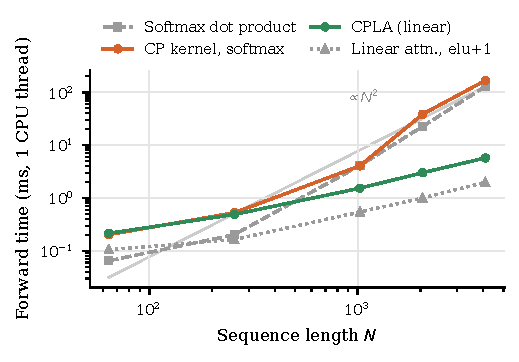
\includegraphics[width=\columnwidth]{figures/timing.pdf}
\caption{Forward time of one attention layer ($d=64$, batch 1, one CPU thread, median of 5 runs) versus sequence length.}
\label{fig:timing}
\end{figure}

Fig.~\ref{fig:timing} confirms the cost analysis. Softmax dot-product attention and the pairwise CP kernel grow quadratically, taking 129 and 167~ms at $N=4{,}096$. \cpla{} grows linearly and takes 5.7~ms, about 22$\times$ faster than softmax attention. Elu$+1$ linear attention is faster still (2.0~ms) because its feature dimension is 16 rather than $4^n=256$, but it fails the matching tasks (Table~\ref{tab:accuracy}). The simulated quantum layer, which shares the pairwise structure, takes 181~ms; on hardware it would instead need $N^2\approx1.7\times10^7$ overlap circuits.

\subsection{Trainability of the Quantum Layer}
\label{sec:trainability}

\begin{figure}[t]
\centering
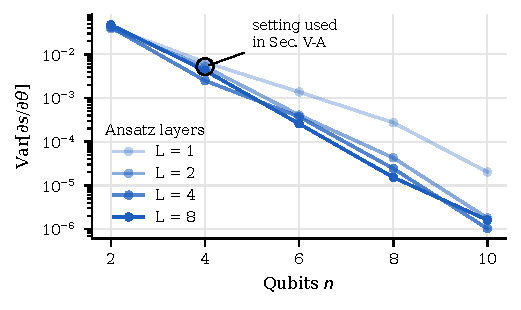
\includegraphics[width=\columnwidth]{figures/gradvar.pdf}
\caption{Variance of $\partial s/\partial\theta_{Q,1}$ at uniformly random parameters (200 samples per point) versus qubit count, for ansatz depths $L\in\{1,2,4,8\}$.}
\label{fig:gradvar}
\end{figure}

Gradient variance at random parameters falls roughly exponentially with $n$ (Fig.~\ref{fig:gradvar}), from about $4\times10^{-2}$ at $n=2$ to about $10^{-6}$ at $n=10$ for $L\ge2$, as expected for a global observable~\cite{cerezo2021cost}. A typical gradient of $10^{-3}$ would need on the order of $10^5$ shots per component to resolve. Depth matters far less than width. Training starts near the identity ($\theta\sim0.1$), which avoids the plateau at initialization for small $n$ but does not remove it as $n$ grows.

\begin{table}[t]
\caption{Two-Pairs Accuracy vs.\ Qubit Count ($L=2$, 3 Seeds)}
\label{tab:qubits}
\centering
\begin{tabular}{@{}cccc@{}}
\toprule
$n$ & Quantum & Dot product ($d_k{=}n$) & Quantum params \\
\midrule
2 & .790$\pm$.073 & .669$\pm$.053 & 587 \\
4 & \textbf{.926}$\pm$.057 & .693$\pm$.010 & 629 \\
6 & .736$\pm$.017 & .710$\pm$.045 & 671 \\
8 & .806$\pm$.097 & .664$\pm$.044 & 713 \\
\bottomrule
\end{tabular}
\end{table}

Larger registers do not improve accuracy (Table~\ref{tab:qubits}); the best result is at $n=4$. This matches the shrinking gradients, though three seeds cannot separate the effects cleanly.

\subsection{Robustness to Shot Noise}

\begin{figure}[t]
\centering
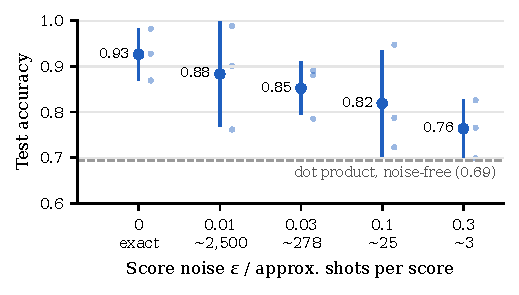
\includegraphics[width=\columnwidth]{figures/noise.pdf}
\caption{Two-pairs accuracy of the quantum layer under simulated shot noise (mean $\pm$ std., 3 seeds; small markers are seeds). Dashed: noise-free dot-product attention on the same seeds.}
\label{fig:noise}
\end{figure}

Accuracy falls from 0.93 with exact scores to 0.76 at about three shots per score (Fig.~\ref{fig:noise}), remaining above the noise-free dot-product baseline (0.69) on average. Seed-to-seed spread is large, so the values indicate a trend.

% ===========================================================================
\section{Discussion and Limitations}
% ===========================================================================

\textit{What transfers to classical Transformers.} The CP kernel is a cheap, exact, bounded similarity with a sharp peak at matching inputs. Through \cpla{} it gives linear-time attention that succeeds on matching tasks where standard linear attention fails. This is the practical outcome of the study, and it requires no quantum hardware.

\textit{What does not.} At the sizes where quantum fidelity attention trains, it is classically simulable, and Proposition~\ref{prop:lin} makes simulation cheaper in $N$ than hardware execution. At sizes where simulation would be hard, gradients have already vanished. A quantum advantage would need encodings whose fidelity resists classical evaluation together with local observables that avoid barren plateaus, a combination that recent theory suggests is difficult~\cite{cerezo2025simulability}.

\textit{Limitations.} The matching tasks are synthetic and favor kernels that peak at equal inputs. SST-2 is a single, short-sequence benchmark, and our models are small single-layer classifiers rather than full Transformers. The exponential feature dimension ($4^n$, or $3^n$ for the CP kernel) restricts \cpla{} to few features per head; multi-head and deeper variants remain to be tested. The noise model covers shot noise on forward scores only, and no experiments ran on quantum hardware. The qubit and noise sweeps use three seeds.

% ===========================================================================
\section{Conclusion}
% ===========================================================================

Quantum fidelity attention outperforms dot-product attention on token-matching tasks, but the advantage comes from a kernel that is exactly computable classically. For angle-encoded states the fidelity is a cosine-product kernel, and any fidelity attention linearizes through an explicit $4^n$-dimensional feature map. The resulting layer, \cpla, matches the quantum model on matching tasks at linear cost and about 22$\times$ the speed of softmax attention at 4{,}096 tokens. On SST-2 the kernel-based layers trail dot-product attention, so the CP kernel is best viewed as a specialized similarity for matching-type structure. Future work should test \cpla{} in multi-head, multi-layer Transformers and on long-range benchmarks, and should look for quantum encodings that resist the reduction presented here.

\section*{Code Availability}
The Qiskit reference implementation with parameter-shift autograd, the statevector simulator, all attention variants and raw results are available at \url{https://github.com/Chandra953/Quantum-Fidelity-Attention}.
Experiments used PyTorch 2.14 and Qiskit 2.5 on a two-core CPU.

\section*{Disclosure of AI Assistance}
Generative AI tools were used to assist with code development, experiment design and drafting of this manuscript. The author reviewed, verified and takes full responsibility for all content.

\bibliographystyle{IEEEtran}
\bibliography{refs}

\end{document}
